% !TEX encoding = UTF-8
% !TEX TS-program = pdflatex
% !TEX root = ../tesi.tex

%**************************************************************
\chapter{Implementazione e documentazione}
\label{cap:implementazione-documentazione}
%**************************************************************

\intro{In questo capitolo viene illustrato il processo di implementazione della soluzione trovata e la stesura della documentazione relativa.}


\section{Configurazione Monokee}
All'interno dell'ambiente di test di Monokee, tramite l'interfaccia web, ho creato una nuova applicazione OAuth2 ed un nuovo OpenID Connect provider, che fornisse gli end-point per l'autenticazione via OIDC.


\section{Configurazione FreeIPA}
Da FreeIPA, ho proceduto a configurare un nuovo Identity Provider server, tramite la sezione della GUI di cui sopra, inserendo tutte i metadati richiesti, facendo riferimento all'applicazione OAuth2 creata su Monokee e agli end-point forniti dall'OpenID provider configurato precedentemente.

Successivamente, ho creato un utente FreeIPA che utilizzasse come unico metodo di autenticazione quella tramite Identity Provider esterno (\emph{External IdP}), scegliendo Monokee come IdP e come identificatore il mio indirizzo e-mail istituzionale, già associato al mio account Monokee, per poter eseguire l'accesso via SSO con le mie credenziali.  

Configurata correttamente l'infrastruttura di autenticazione sia su Monokee che su FreeIPA, ho proceduto a verificarne il funzionamento seguendo le indicazioni della documentazione relativa: dapprima, ho generato un file per l'autenticazione tramite canale FAST con il comando \texttt{kinit -n -c ./fast.ccache}; successivamente, ho richiesto l'autenticazione anonima tramite PKINIT con il comando \texttt{kinit -T ./fast.ccache monokee1}; a questo punto, viene eseguito il flusso di OIDC e viene mostrato un URL al quale autenticarsi tramite SSO di Monokee; ad autenticazione eseguita, basta tornare sul terminale e premere invio per completare l'autenticazione.

Per verificare la corretta autenticazione ho poi lanciato il comando \texttt{klist}, che mostra i ticket Kerberos richiesti, e controllato che l'utente attuale fosse lo stesso con cui volevo autenticarmi e che il ticket fosse valido.  

\begin{figure}[!h] 
    \centering 
    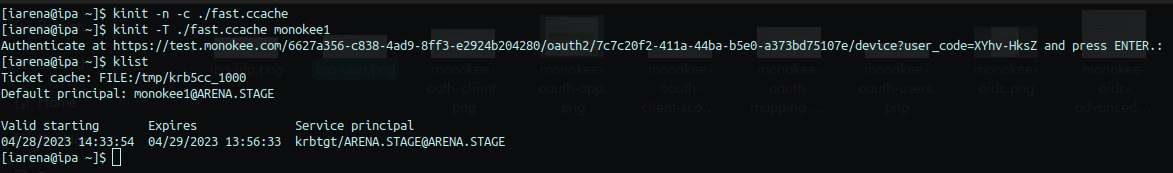
\includegraphics[width=\columnwidth]{ipa-cli} 
    \caption{Autenticazione con Monokee SSO tramite FreeIPA da CLI}
    \label{fig:ipa-cli}
\end{figure}

% Mettere la roba dell'autenticazione con google ecc

\section{Problematiche riscontrate}

Durante l'integrazione dell'SSO tramite FreeIPA, nonché già dal processo di configurazione dello stesso, ho riscontrato numerose problematiche.

In primis, a rendere il processo più faticoso del previsto, è stata la mancanza di una  documentazione esaustiva e di informazioni utili in rete in merito alla risoluzione degli errori, dovuta probabilmente alla userbase di FreeIPA, che, benché tale servizio sia lo standard in ambito IAM, è alquanto ridotta.

In secondo luogo, ho riscontrato errori di inconsistenza piuttosto limitanti tra i registri di FreeIPA e quelli di sistema, oltre che difetti di compatibilità della piattaforma con alcune versioni di CentOS e RHEL.

Infine, l'autenticazione di FreeIPA tramite MOnokee SSO non riesce a sovrascrivere quella di UNIX quando si vuole raggiungere una macchina tramite SSH su un utente Monokee già configurato sul server. 

\section{Sviluppi futuri}
A partire dai risultati che ho ottenuto durante l'attività di stage, gli sviluppi futuri possibili sono molteplici.

Innanzitutto, comincerei con il risolvere il problema legati all'accesso alle macchine con il server di FreeIPA installato tramite SSH su un utente di FreeIPA, e, dunque, per mezzo del Single Sign-On di Monokee. L'SSO, difatti, viene bypassato e viene richiesta la password dell'utente, la quale, di fatto, non esiste perché non è utilizzata da FreeIPA sugli utenti da autenticare con Monokee. 

Dunque, andrei a verificare le impostazioni attive nei file di configurazione di SSH, come \texttt{/etc/ssh/sshd\_config}.
\\ \\
Risolto questo problema e avendo, quindi, una macchina a cui è possibile accedere tramite SSH direttamente con un utente Monokee, il prossimo passo potrebbe essere quello di predisporre delle macchine server con le risorse dell'azienda e fornirne l'accesso 
direttamente da Monokee, utilizzando un servizio come Apache Guacamole.

In questo modo, un utente Monokee privilegiato potrebbe accedere a delle macchine server gestire accessi, privilegi ed altro, oppure, nel caso di un utente subordinato, accedere a delle macchine client, gestite da quella server.
\section{Documentazione}

L'azienda ha richiesto la redazione di una guida che illustrare il processo di configurazione del server FreeIPA e dei sistemi di Monokee per l'integrazione del Single Sign-On sulle macchine UNIX, per fornire una base documentativa per facilitare le future progressioni e sperimentazioni relative. Ho steso tale documentazione in formato Markdown, versionando il codice sul repository GitHub aziendale fornito da \myAzienda.